%
%  hume.two
%
%  Created by Mark Eli Kalderon on 2007-08-03.
%  Copyright (c) 2007 Mark Eli Kalderon. All rights reserved.
%
%  Beamer

% Definitions and macros
\newcommand{\change}{\textcolor{blue}{\textbf{CHANGE SLIDE}}}
\newcommand\myauthor{Mark Eli Kalderon} 
\newcommand\mytitle{Introduction to Moral Philosophy}
\newcommand\mysubtitle{Hume}
\newcommand\myinstitution{University College London}
\newcommand\myurl{http://markelikalderon.com/teaching/}

% Packages specific to lecture notes
\mode<article>{
    \usepackage{palatino}
}

% Packages specific to beamer presentation
\mode<presentation>{
    \usetheme{Darmstadt}
    \setbeamercovered{transparent}
    \pgfdeclareimage[height=0.5cm]{university-logo}{../../../graphics/logo_sml_blk}
    \logo{\pgfuseimage{university-logo}}
}

% Packages common to lecture notes and beamer presentation
\usepackage{pgf}
\usepackage{tikz}
\usepackage{hyperref}

\setjobnamebeamerversion{hume.two.beamer}

\title{\mytitle}
\subtitle{\mysubtitle}

\author{\myauthor\\
\url{\myurl}}
\institute{\myinstitution}

% \date[Short Occasion] % (optional)
% {Date / Occasion}

\begin{document}

% TODO: add CHANGE SLIDEs throughout

\frame{\maketitle}

\section{Review}\label{sec:review} % (fold)

\change

% TODO: Notes for review

\change

% \textbf{See Figure~\ref{fig:slide1}}
% 
% \begin{figure}[ht]
%     \begin{center}
%         \includeslide[height=5cm]{slide1<1>}
%     \end{center}
%     \caption{Main Points from Last Time}
%     \label{fig:slide1}
% \end{figure}

\frame<presentation>[label=slide1]{
    \frametitle{Main Points from Last Time}
        \begin{columns}
            \begin{column}{3cm}
                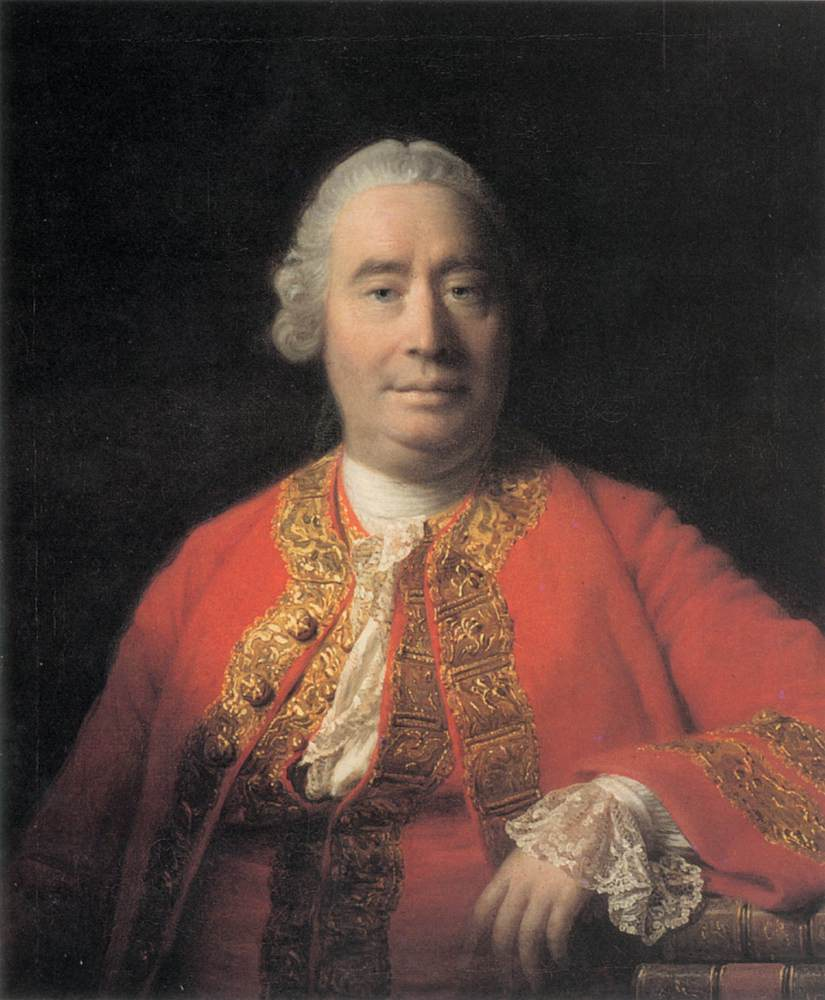
\includegraphics[height=4cm]{../../../graphics/hume.jpg}
            \end{column}
            \begin{column}{7cm}
                \begin{itemize}
                    \item The Anatomy of Morals
                    \item The First Principle in the Science of Human Nature
                    \item The Connexion or Association of Ideas
                \end{itemize}
            \end{column}
        \end{columns}
}

% section review (end)

\section{The Passions}\label{sec:the_passions} % (fold)

In Book I of the \emph{Treatise} Hume makes three important claims about the passions:

\begin{itemize}
    \item The passions are impressions of reflection.
    \item Many of the impressions of reflection derive from ideas that in turn derive from certain bodily sensations such as pain or pleasure.
    \item In addition to love, hatred, pride, etc., the passions include desires.
\end{itemize}

\change

% \begin{figure}[ht]
%     \begin{center}
%         \includeslide[height=5cm]{slide2<1>}
%     \end{center}
%     \caption{The Passions in Book I}
%     \label{fig:slide2}
% \end{figure}

\frame<presentation>[label=slide2]{
    \frametitle{The Passions in Book I}
        \begin{columns}
            \begin{column}{3cm}
                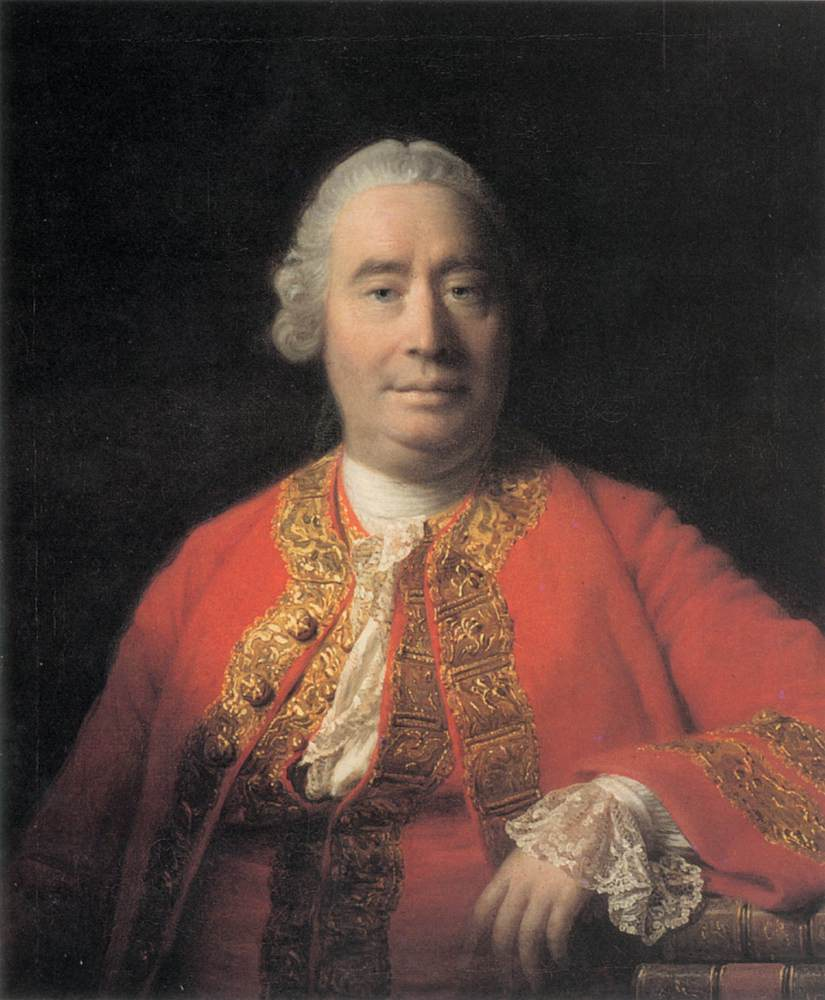
\includegraphics[height=4cm]{../../../graphics/hume.jpg}
            \end{column}
            \begin{column}{7cm}
                \begin{itemize}
                    \item The passions are impressions of reflection.
                    \item Many of the impressions of reflection derive from ideas that in turn derive from certain bodily sensations such as pain or pleasure.
                    \item In addition to love, hatred, pride, etc., the passions include desires.
                \end{itemize}
            \end{column}
        \end{columns}
}

In Book II of the \emph{Treatise} distinguishes passions according to how they originate:

\begin{itemize}
    \item \textbf{Direct passions} derive immediately from pleasure or pain. \change
    \item \textbf{Indirect passions} like direct passions derive from pleasure and plain but not immediately. \change
    \item \textbf{Original passions} do not derive from pleasure or pain, although when acted upon they produce pleasure or pain. \change
\end{itemize}

Original passions are implanted instincts. They do not derive from pleasure or pain, but when acted upon they produce pleasure or pain. Bodily appetites such as hunger are examples of original passions. Other original passions include benevolence, kindness towards children, the desire to punish enemies, and to aid friends. \textbf{CHANGE SLIDE}

In contrast, direct passions derive immediately from pleasure or pain. Thus for example, the pain we experience from the loss of a loved one gives rise to grief, just as the pleasure that results from the charm of a loved one gives rise to joy. Other direct passions include, desire and aversion, hope and fear. \textbf{CHANGE SLIDE}

Indirect passions derive from pleasure and pain, just like direct passions, but not immediately. Indirect passions include pride and humility, love and hate, moral approbation and disapprobation, the sense of beauty and deformity.

The bulk of Book II is dedicated to discussing indirect passions, since these are governed by a limited number of general principles and so exemplify the new science of human nature. One of Hume's aims is to demonstrate what can be done in the new science and so vouchsafe his claim to being the Neton of the Mind (pictured here). In contrast with metaphysical speculation about the supersensible nature of things which warrants only skeptical despair, progress can genuinely be made in moral philosophy. \change

% See Figure~\ref{fig:slide3}
% 
% \begin{figure}[ht]
%     \begin{center}
%         \includeslide[height=5cm]{slide3<3>}
%     \end{center}
%     \caption{The Origin of the Passions}
%     \label{fig:slide3}
% \end{figure}

\frame<presentation>[label=slide3]{
    \frametitle{The Origin of the Passions}
        \begin{columns}
            \begin{column}{3cm}
                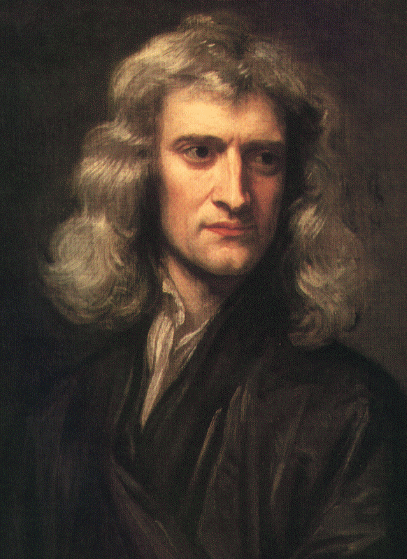
\includegraphics[height=4cm]{../../../graphics/newton.jpg}
            \end{column}
            \begin{column}{7cm}
                \begin{itemize}
                    \item<1-> \alert{Direct passions} derive immediately from pleasure or pain.
                    \item<2-> \alert{Indirect passions} like direct passions derive from pleasure and plain but not immediately.
                    \item<3-> \alert{Original passions} do not derive from pleasure or pain, although when acted upon they produce pleasure or pain.
                \end{itemize}
            \end{column}
        \end{columns}
}

In addition to distinguishing the passions according to their origin, Hume also distinguishes passions according to their turbulence and felt intensity. Turbulence and felt intensity admit of degrees, and so the distinction is not precise (as Hume himself recognizes). Nevertheless, a distinction can be made between:

\begin{itemize}
    \item Calm passions
    \item Violent passions.
\end{itemize}

Calm passions ``though they be real passions produce little emotion in the mind and are more known by their effects than by the immediate feeling of sensation'' (\emph{Treatise}, 2.3.3.8). In this way, they differ from violent passions, such as resentment, which can be known by immediate feeling or sensation. Calm passions include benevolence and the sense of beauty and deformity. Violent passions include love and hatred, grief and joy, pride and humility. \change

Finally, Hume distinguishes passions according to their causal influence:

\begin{itemize}
    \item Strong passions exert a steady and controlling influence over reasoning and conduct.
    \item Weak passions exert an unsteady and less controlling influence over reasoning and conduct.
\end{itemize}

Again, causal influence is a matter of degree and so this distinction is not precise (as Hume himself recognizes). Unlike the distinction between calm and violent passions, the distinction between strong and weak passions does not pertain to the nature of the passions. Benevolence is by nature calm, but it may exert a steady and controlling influence over the conduct of one person but not another. The difference between the strength of passions is a difference in the role they play in the system of the passions. It is a difference, not in the nature of the passion, but in the character of the passionate subject. \change

% See Figure~\ref{fig:slide4}
% 
% \begin{figure}[ht]
%     \begin{center}
%         \includeslide[height=5cm]{slide4<2>}
%     \end{center}
%     \caption{Phenomenology and Causal Influence}
%     \label{fig:slide4}
% \end{figure}

\frame<presentation>[label=slide4]{
    \frametitle{Phenomenology and Causal Influence}
        \begin{columns}
            \begin{column}{3cm}
                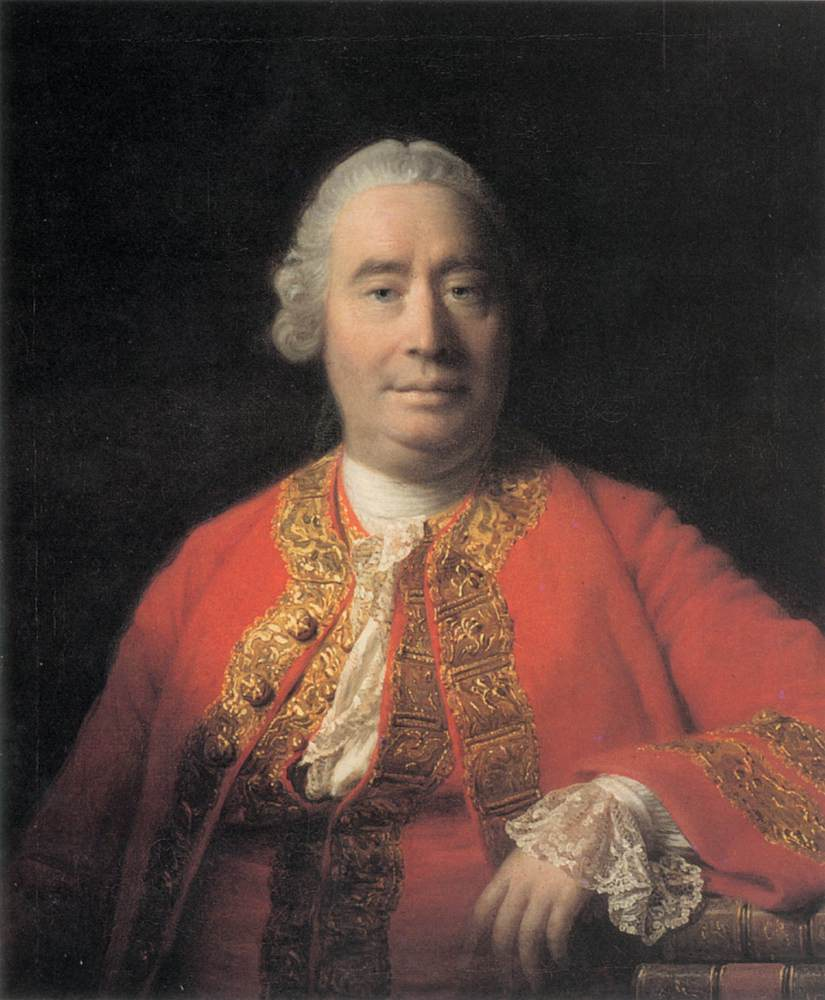
\includegraphics[height=4cm]{../../../graphics/hume.jpg}
            \end{column}
            \begin{column}{7cm}
                Hume also distinguishes passions according to their turbulence \& felt intensity \& their causal influence:
                \begin{itemize}
                    \item<1-> Passions are \alert{calm} or \alert{violent}
                    \item<2-> Passions are \alert{strong} or \alert{weak}
                \end{itemize}
            \end{column}
        \end{columns}
}

Putting these distinctions together, we get the following:

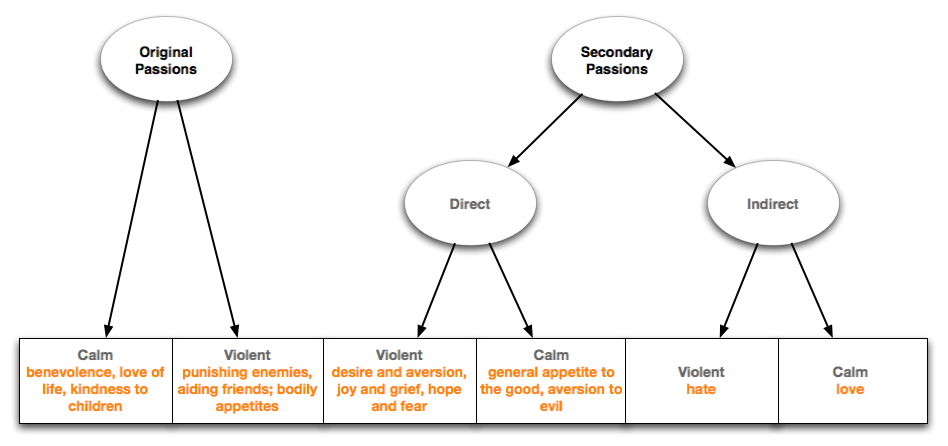
\includegraphics[width=\textwidth]{../../../graphics/passions.jpg}

\change

% See Figure~\ref{fig:slide5}
% 
% \begin{figure}[ht]
%     \begin{center}
%         \includeslide[height=5cm]{slide5<1>}
%     \end{center}
%     \caption{The Taxonomy of the Passions}
%     \label{fig:slide5}
% \end{figure}

\frame<presentation>[label=slide5]{
    \frametitle{The Taxonomy of the Passions}
        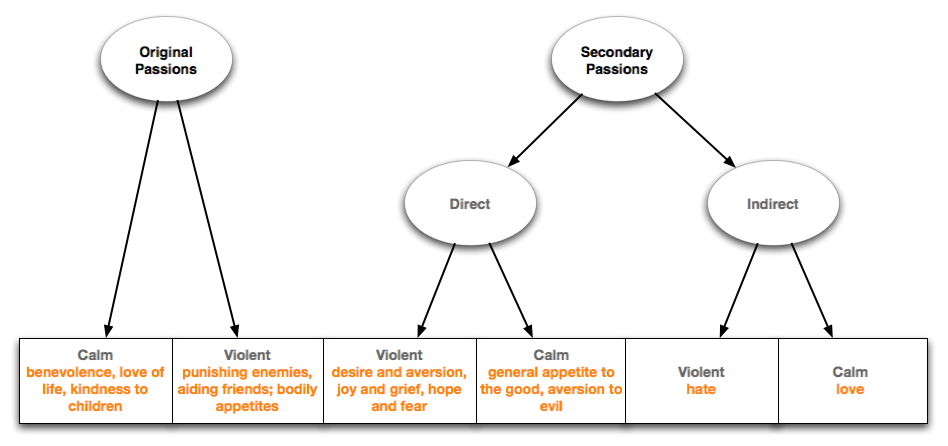
\includegraphics[width=\textwidth]{../../../graphics/passions.jpg}
}

% section the_passions (end)

\section{The Double Relation of Ideas and Impressions}\label{sec:the_double_relation_of_ideas_and_impressions} % (fold)

Passions are impressions. Certain important passions, such as pride and humility, are simple impressions. Being simple, these impressions cannot be defined or otherwise analyzed into their constituent parts for they have no such parts. However, this does not mean that the moral scientist can say nothing about them. The moral scientist can enumerate ``such circumstances, as attend them'' (\emph{Treatise}, 2.1.2.1). That is, the moral scientist can describe the circumstances that give rise to these simple impressions and so discover the limited number of principles that govern them. \change

Pride is ``that agreeable impression that arises in the mind, when the view either of our virtue, beauty, riches or power makes us satisy'd with ourselves'' (\emph{Treatise}, 2.1.7.8). Humility, in contrast, is a disagreeable impression that arises in the mind when the view of our virtue, beauty, riches or power makes us dissatisfied with ourselves. Pride and humility are thus contrary impressions. \change

These passions are contrary; nevertheless, they have the same \emph{object}. According to Hume, the passions of pride and humility always have the self as their object. The object of pride or humility is the very person who is feeling these passions. \change

Just as pride and humility have the same object, they also have the same kind of \emph{causes}. Such causes are \emph{subjects} with particular \emph{qualities}. So if owning a beautiful house occasions pride, the cause of this passion is the beautiful house, the house being the subject, and its beauty being the particular quality. \change

% \textbf{See Figure~\ref{fig:slide6}}
% 
% \begin{figure}[ht]
%     \begin{center}
%         \includeslide[height=5cm]{slide6<4>}
%     \end{center}
%     \caption{Pride \& Humility}
%     \label{fig:slide6}
% \end{figure}

\frame<presentation>[label=slide6]{
    \frametitle{Pride \& Humility}
        \begin{itemize}
            \item<1-> Pride \& humility are \alert{simple impressions}
            \item<2-> Pride is an \alert{agreeable impression}, a kind of pleasure; humility is a \alert{disagreeable impression}, a kind of pain
            \item<3-> Pride \& humility have the same object: the \alert{self}
            \item<4-> The same kind of \alert{subjects} \& \alert{qualities} give rise to pride \& humility 
        \end{itemize}
}

Just as the contrary passions of pride and humility have the same object and kind of causes, they also depend upon certain principles of association. Recall, ideas that are related by resemblance, contiguity, or causation are naturally associated as if by a force analogous to gravity or magnetism:

\begin{quote}
    \'Tis impossible for the mind to fix itself steadily upon one idea for any considerable time; nor can it by its utmost effort ever arrive at such a constancy. But however changeable our thoughts may be, they are not entirely without rule and method in their changes. The rule, by which they proceed, is to pass from one object to what is resembling, contiguous to, or produc'd by it. When one idea is present to the imagination, any other, united by these relations, naturally follows it, and enters with more facility by means of that introduction. (\emph{Treatise}, 2.1.4.2)
\end{quote}

In addition, Hume observes that impressions are also naturally associated. Whereas the natural association of ideas proceeds through the relations of resemblance, contiguity, and causation, the natural association of impressions proceeds only through the relation of resemblance. The experience of a disagreeable impression will naturally lead us to experience other disagreeable impressions. ``Grief and disappointment give rise to anger, anger to envy, envy to malice, and malice to grief again, till the whole circle be compleated'' (\emph{Treatise}, 2.1.4.3).

Thus Hume distinguishes between two kinds of association:

\begin{itemize}
    \item \emph{The Association of Ideas} whose principles include resemblance, contiguity, and causation.
    \item \emph{The Association of Impressions} whose sole principle is resemblance.
\end{itemize}

\change

% See Figure~\ref{fig:slide7}
% 
% \begin{figure}[ht]
%     \begin{center}
%         \includeslide[height=5cm]{slide7<1>}
%     \end{center}
%     \caption{Two Kinds of Association}
%     \label{fig:slide7}
% \end{figure}

\frame<presentation>[label=slide7]{
    \frametitle{Two Kinds of Association}
        \begin{columns}
            \begin{column}{3cm}
                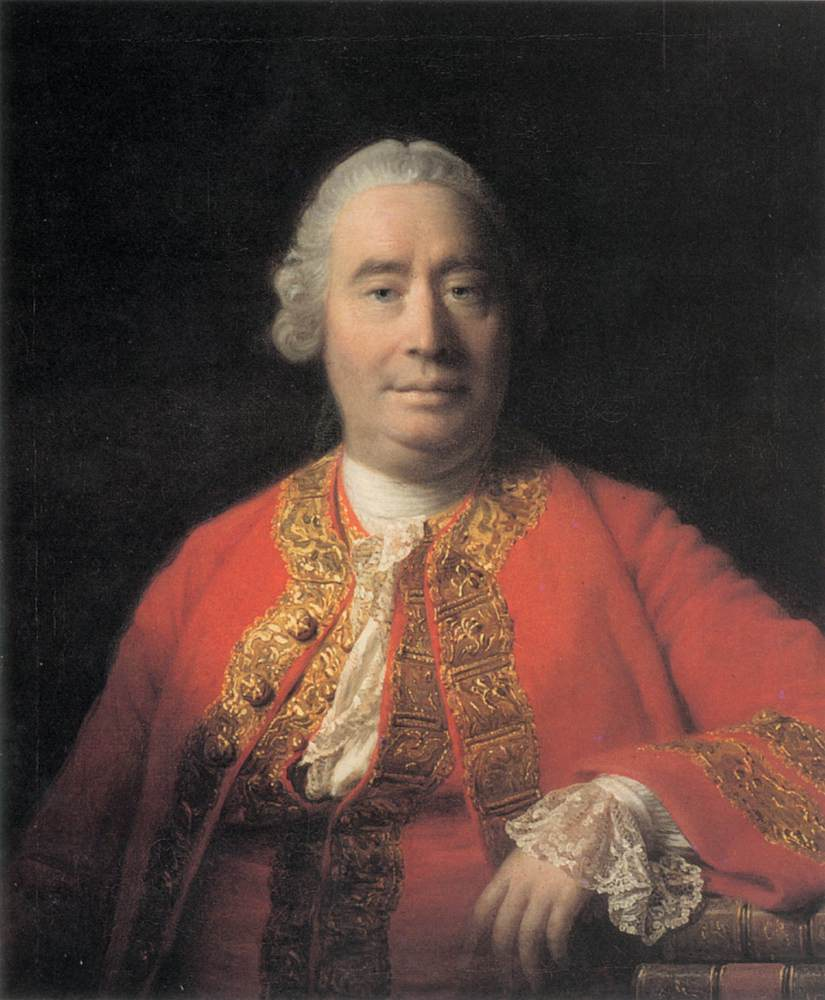
\includegraphics[height=4cm]{../../../graphics/hume.jpg}
            \end{column}
            \begin{column}{7cm}
                \begin{itemize}
                    \item \alert{The Association of Ideas} whose principles include resemblance, contiguity, and causation.
                    \item \alert{The Association of Impressions} whose sole principle is resemblance.
                \end{itemize}
            \end{column}
        \end{columns}
}

Having established that pride is an agreeable impression and humility disagreeable, and having distinguished the cause and object of these passions, and having observed that impressions are naturally associated just as ideas are, Hume is now in a position explain how these passions originate:

\begin{quote}
    If I compare, therefore, these two \emph{establish'd} properties of the passions, \emph{viz}. their object, which is self, and their sensation, which is either pleasant or painful, to the two \emph{suppos'd} properties of the causes, viz. their relation to self, and their tendency to produce a pain or a pleasure, independent of the passion; I immediately find, that taking these suppositions to be just, the true system breaks in upon me with irrresistable evidence. The cause, which excites the passion, is related to the object, which nature has attributed to the passion; the sensation, which the cause separately produces, is related to the sensation of the passion; From this double relation of ideas and impressions, the passion is deriv'd. The one idea is easily converted into its correlative; and the one impression into that, which resembles and corresponds to it: With how much greater facility must this transition be made, where these movements mutually assist each other, and the mind receives a double impulse from the relations both of its impressions and ideas? (\emph{Treatise}, 2.1.5.5)
\end{quote}


Hume's exposition of ``the true system'' is admittedly dense, but the idea seems to be this: Pride and humility depend on a ``double relation of ideas and impressions''. The cause of pride (a certain subject in which a particular quality inheres) affects a person by means of the idea that person has of it. A person's idea of the subject, because the subject is his, by the association of ideas, occasions his idea of himself. Thus the subject brings to mind what is always the object of pride, the person who feels that passion. The cause of pride also affects a person by means of the impression that person has of it. The quality of the subject, being positive, gives a person pleasure. This impression, because it resembles the pleasure of pride, by the association of impressions, occasions pride. \change

% \textbf{See Figure~\ref{fig:slide8}}
% 
% \begin{figure}[ht]
%     \begin{center}
%         \includeslide[height=5cm]{slide8<1>}
%     \end{center}
%     \caption{Treatise 2.1.5.5}
%     \label{fig:slide8}
% \end{figure}

\frame<presentation>[label=slide8]{
    \frametitle{Treatise 2.1.5.5}
        \small{If I compare, therefore, these two \emph{establish'd} properties of the passions, \emph{viz}. their object, which is self, and their sensation, which is either pleasant or painful, to the two \emph{suppos'd} properties of the causes, viz. their relation to self, and their tendency to produce a pain or a pleasure, independent of the passion; I immediately find, that taking these suppositions to be just, the true system breaks in upon me with irrresistable evidence. The cause, which excites the passion, is related to the object, which nature has attributed to the passion; the sensation, which the cause separately produces, is related to the sensation of the passion; From this double relation of ideas and impressions, the passion is deriv'd. The one idea is easily converted into its correlative; and the one impression into that, which resembles and corresponds to it: With how much greater facility must this transition be made, where these movements mutually assist each other, and the mind receives a double impulse from the relations both of its impressions and ideas?}
}

An example will help. Suppose I consider my beautiful house. Since the beautiful house is \emph{mine}, my idea of the house, by the association of ideas, tends to occasion my idea of myself. Moreover, the house, since it has a positive quality, beauty, occasions a particular pleasure. And this pleasure, since it resembles the agreeable impression of pride, by the natural association of impressions, tends to occasion that passion. Thus the association of impressions and ideas works together to give rise to the passion of pride. This process is represented in the diagram pictured here: \change

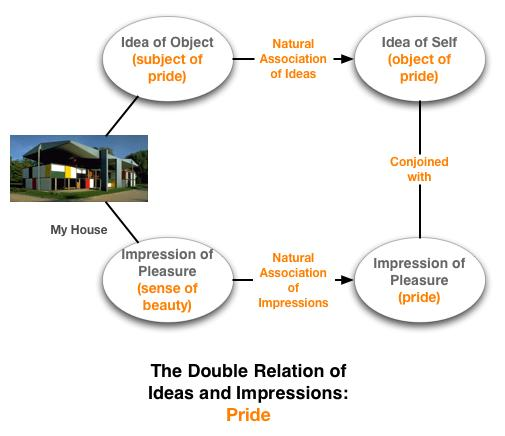
\includegraphics[width=\textwidth]{../../../graphics/pride.jpg}

% See Figure~\ref{fig:slide9}
% 
% \begin{figure}[ht]
%     \begin{center}
%         \includeslide[height=5cm]{slide9<1>}
%     \end{center}
%     \caption{Double Relation of Ideas and Impressions}
%     \label{fig:slide9}
% \end{figure}

\frame<presentation>[label=slide9]{
    \frametitle{Double Relation of Ideas and Impressions}
        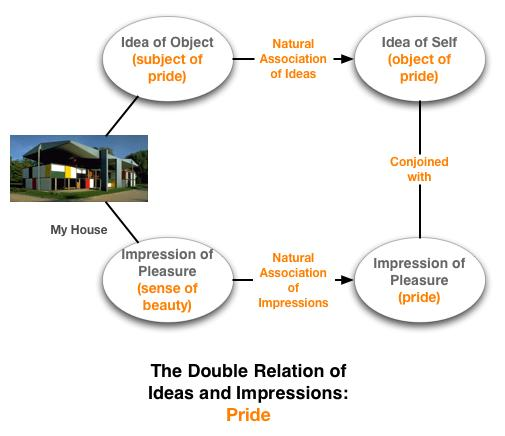
\includegraphics[width=\textwidth]{../../../graphics/pride.jpg}
}

% section the_double_relation_of_ideas_and_impressions (end)

\section{Sympathy}\label{sec:sympathy} % (fold)

Hume observes that being esteemed by another gives rise to pride. This raises a puzzle about what Hume calls the \emph{secondary causes} of pride and humility. How can the pleasure that another person feels cause pride in oneself? When pride arises from the possession of a beautiful house, it is the agreeable sensation of the house, the sense of its beauty, that, by the association of impressions, tends to produce the agreeable impression of pride. But when pride arises from the esteem of others, it is not the person's pleasure that gives rise to pride, but the pleasure of another. The problem for Hume's account is that the association of impressions (whereby impressions tend to produce other impressions that resemble them) only works \emph{intra}personally---it is a principle that coordinates the impressions within the mind of a single person. \change

% \textbf{See Figure~\ref{fig:slide10}}
% 
% \begin{figure}[ht]
%     \begin{center}
%         \includeslide[height=5cm]{slide10<1>}
%     \end{center}
%     \caption{The Association of Impressions}
%     \label{fig:slide10}
% \end{figure}

\frame<presentation>[label=slide10]{
    \frametitle{Association of Impressions}
        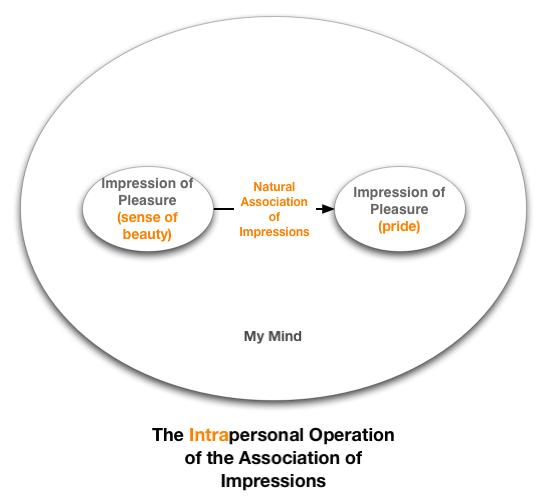
\includegraphics[width=\textwidth]{../../../graphics/intrapersonal.jpg}
}

In the case of secondary causes of pride, Hume needs a principle that works \emph{inter}personally---a principle that coordinates the impressions within the minds of different persons. According to Hume, \emph{sympathy} is the needed interpersonal principle of coordination.

Hume's usage of ``sympathy'' is thus at variance with the vulgar's. Very often, when the vulgar speak of sympathy, they have in mind a particular feeling, what Hume would describe as pity or compassion. However, as Hume uses the term, sympathy is not a sentiment; it is not a passion that one feels. Rather, sympathy is a principle that coordinates the impressions of different people:

\begin{quote}
    When any affection is infus'd by sympathy, it is first known only by its effects, and by those external signs in the countenance and conversation, which convey an idea of it. The idea is presently converted into an impression, and acquires such a degree of force and vivacity, as to become the very passion itself, and produce an equal emotion, as any original affection.
\end{quote}

How does this work?

Like the principles involved in the association of ideas, sympathy is a fundamental principle of human nature. Nevertheless, its operation depends in part on human perceptions and the relations of resemblance, contiguity, and causation between them. This dependency, however, is to be expected. Hume explains:

\begin{quote}
    Our affections depend more upon ourselves, and the internal operations of the mind, than any other impressions; for which reason they arise more naturally from the imagination, and from every lively idea we form of them. (\emph{Treatise}, 2.1.11.7)
\end{quote}

How, then, do the principles of resemblance, contiguity, and causation aid in transforming an idea of a passion into the passion itself? Hume begins by observing that each of us possess a lively impression of ourselves:

\begin{quote}
    \'Tis evident, that the idea, or rather impression of ourselves is always intimately present with us, and that our consciousness gives us so lively conception of our own person, that \'tis not possible to imagine, that any thing can in this particular go beyond it. (\emph{Treatise}, 2.1.11.4)
\end{quote}

So lively is this impression of ourselves, that it can lend its force or vivacity to impressions and ideas related to it: ``Whatever object, therefore, is related to ourselves must be conceiv'd with a like vivacity of conception, according to the foregoing principles'' (\emph{Treatise}, 2.1.11.4).

So suppose my friend has received good news and this has made him happy. This passion, happiness, affects his appearance and behavior: He has a cheerful countenance, a bright smile, and a lively step. When I perceive his appearance and behavior, I take these as a sign of his happiness since I know from experience that such appearance and behavior is typically caused by that passion. Now my friend is related to me by resemblance and contiguity. My friend resembles me and not merely in the general manner in which all humans resemble one another. More than this, we share certain interests and concerns together. Moreover, he is contiguous with me---he has just greeted me to convey his good news. I have formed an idea of my friend's happiness. Since he is \emph{my} friend, related to me by resemblance and contiguity, my lively conception of myself lends its force and vivacity to my idea of my friend's happiness and converts this idea into the corresponding impression. I come to feel happy myself and so share in my friend's happiness. \change

% \textbf{See Figure~\ref{fig:slide11}}
% 
% \begin{figure}[ht]
%     \begin{center}
%         \includeslide[height=5cm]{slide11<1>}
%     \end{center}
%     \caption{Sympathy}
%     \label{fig:slide11}
% \end{figure}

\frame<presentation>[label=slide11]{
    \frametitle{Sympathy}
        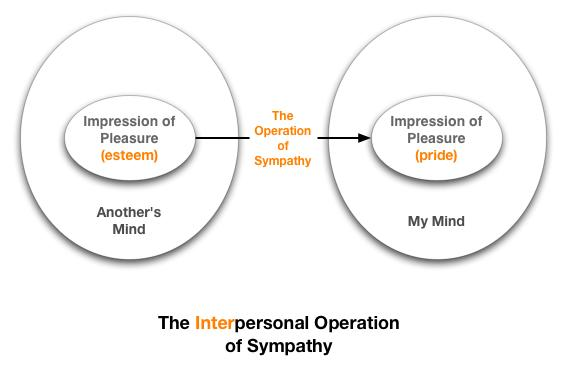
\includegraphics[width=\textwidth]{../../../graphics/interpersonal.jpg}
}

Though Hume sometimes speaks of sympathy as a \emph{principle of communication} it is perhaps more aptly described as a \emph{principle of coordination}. In the example above, and in many of Hume's own examples, the passion of one person gives rise to the very same passion in another. The passion has been ``communicated'' from one person to another. This can encourage an interpretation of sympathy as a kind of emotional contagion. Just as contagious disease can be communicated from one person to another, so too can the human passions be communicated from one person to another. However, sympathy can give rise to distinct if complementary passions. Thus, for example, grief in one person can give rise, through the operation of sympathy, to pity in another. Moreover, in the case at hand, esteem in one person can give rise to pride in another. In these cases, the passion of one has not been communicated to another; rather, the passions of each have been coordinated by the mechanism of sympathy.

With the principle of sympathy, the secondary causes of pride are easily explained. If I elicit esteem in another, their idea of me gives rise to that agreeable impression because of some positive quality that I possess. Indeed, the range of qualities for which I may be esteemed is the same range of qualities that I can be proud of. Felt esteem affects the person's appearance and behavior. I take these as a sign for his esteem since I know from experience that such appearance and behavior is typically caused by that passion. I form an idea of the other's pleasure. By the operation of sympathy the idea I form of this agreeable impression is converted into that impression. Moreover, since I am cognizant that I am the object of another's esteem because of certain positive qualities I posses, by the association of ideas, this occasions my idea of myself. I feel pleasure and I am the object of this feeling. This just is the passion of pride. In this way, sympathy can coordinate the distinct if complementary passions of esteem and pride. \change

% See Figure~\ref{fig:slide12}
% 
% \begin{figure}[ht]
%     \begin{center}
%         \includeslide[height=5cm]{slide12<1>}
%     \end{center}
%     \caption{Two Interpretations}
%     \label{fig:slide12}
% \end{figure}

\frame<presentation>[label=slide12]{
    \frametitle{Two Interpretations}
        \begin{itemize}
            \item Sympathy is a \alert{principle of communication}, a kind of emotional contagion. Just as contagious disease can be communicated from one another, so too can human emotion be communicated from one to another
            \item Sympathy is a \alert{principle of coordination}. While some passions can be communicated from one to another, sympathy can give rise to distinct, if complementary passions
        \end{itemize}
}

Sympathy is not a passion as the vulgar speak of it; rather, it is a fundamental principle of human nature that coordinates impressions. Unlike the principles of association, sympathy is an interpersonal as opposed to an intrapersonal principle: Whereas the association of impressions coordinates impressions within the mind of a single person, sympathy coordinates the impressions within the minds of different people. While sympathy can communicate some passions from one person to another, it is better understood as a principle of coordination since it can give rise to distinct if complementary passions in different people. Since it is a fundamental principle of human nature that coordinates the passions felt by oneself with the passions felt by others, it is plausibly the source of the distinction between self and other. It is partly for this reason that sympathy can play the important role that it does play in Hume's account of the virtues. \change

% \textbf{See Figure~\ref{fig:slide13}}
% 
% \begin{figure}[ht]
%     \begin{center}
%         \includeslide[height=5cm]{slide13<1>}
%     \end{center}
%     \caption{Sympathy Summarized}
%     \label{fig:slide13}
% \end{figure}

\frame<presentation>[label=slide13]{
    \frametitle{Sympathy Summarized}
        \begin{itemize}
            \item Sympathy \alert{is not a passion}, it is a fundamental principle that coordinates impressions in different people
            \item Unlike the principles of association, sympathy is an \alert{inter}personal as opposed to \alert{intra}personal principle
            \item Sympathy is a \alert{principle of coordination} rather than a \alert{principle of communication}
        \end{itemize}
}

Love and hate (of which esteem and contempt are species) are in many ways similar to pride and humility:

\begin{itemize}
    \item Love and hate, like pride and humility, are simple impressions and so indefinable.
    \item Love and hate, like pride and humility, are agreeable and disagreeable, respectively.
    \item Love and hate, like pride and humility, are indirect passions that arise through the double relation of ideas and impressions.
\end{itemize}

There is, however, a crucial difference. Whereas pride and humility always take the self as their object, love and hate always take another person as their object: Just as pride is an agreeable impression of oneself, love is an agreeable impression of another; and just as humility is a disagreeable impression of oneself, hatred is a disagreeable impression of another. If we classify indirect passions by whether they are agreeable or disagreeable and whether they take the self or the other as their object, we can taxonomize these passions as pictured. As we will see, this nonaccidentally mirrors the taxonomy of the virtues that Hume will offer. \change

% \textbf{See Figure~\ref{fig:slide14}}
% 
% \begin{figure}[ht]
%     \begin{center}
%         \includeslide[height=5cm]{slide14<1>}
%     \end{center}
%     \caption{The Square of Passions}
%     \label{fig:slide14}
% \end{figure}

\frame<presentation>[label=slide14]{
    \frametitle{The Square of Passions}
        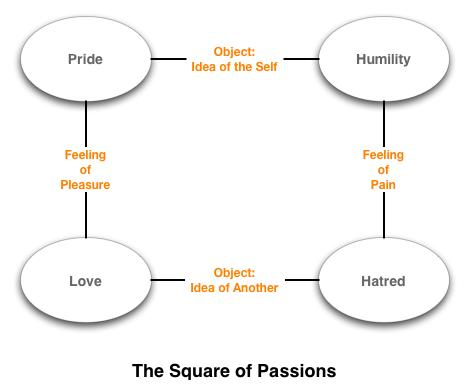
\includegraphics[width=\textwidth]{../../../graphics/square_of_passions.jpg}
}

% section sympathy (end)

\section{Next Time}\label{sec:next_time} % (fold)

\frame<presentation>[label=slide15]{
    \frametitle{Readings for Next Time}
        Covered next lecture:
            \begin{itemize}
                \item 2.3.3
                \item 3.1.1--2
                \item Rawls, Hume II
            \end{itemize}
}

% section next_time (end)

\end{document}
